\documentclass{jsarticle} 
\usepackage[dvipdfmx]{graphicx} 
\usepackage[dvipdfmx]{hyperref}
\usepackage{amsmath}
\usepackage{color}
\usepackage{colortbl}
\usepackage{arydshln}
\usepackage{mathtools}

\newcommand*{\mbold}[1]{\mbox{\boldmath $#1$}}

%\renewcommand*{\labelenumi}{(\arabic{enumi})}

\newcommand*{\transp}[1]{\prescript{t\!}{}{#1}}

\newcommand*{\grad}{{\rm grad}}
\newcommand*{\divg}{{\rm div}}
\newcommand*{\rot}{{\rm rot}}
\newcommand*{\trace}[1]{{\rm tr}\!{#1}}


\title{Theorem1.33 : Gauss's Theorem}

\begin{document}
\maketitle

\begin{abstract}
  閉曲面$S : \mbold{S}(u, v)$に囲まれた領域$V$に対し, $V$内で定義されているベクトル場$\mbold{A}$について, 以下が成り立つ. 
  \begin{eqnarray}
    \int_S \mbold{A}\cdot \mbold{n}dS = \int_V \divg \mbold{A}dV 
  \end{eqnarray}
\end{abstract}

\section{lemma1 : 面積分に対し, 積分領域に, 任意の, 同一形状の表裏面領域を設けても結果が変わらない}
この内容は, Theorem1.32のlemma1の, 面バージョンである. 
ある面$S$上を積分していく, 面経路上に, $S$につながっている, 別の面$S^\prime$を考える. 
図のように, $S$と, $S^\prime$が接触する曲線, もしくは点を含む, $S$上の曲線$C$で, $S$を二分割し, 分割された面を$S_1$, $S_2$と呼ぶことにする. 
\begin{figure}[htbp]
  \begin{center}
    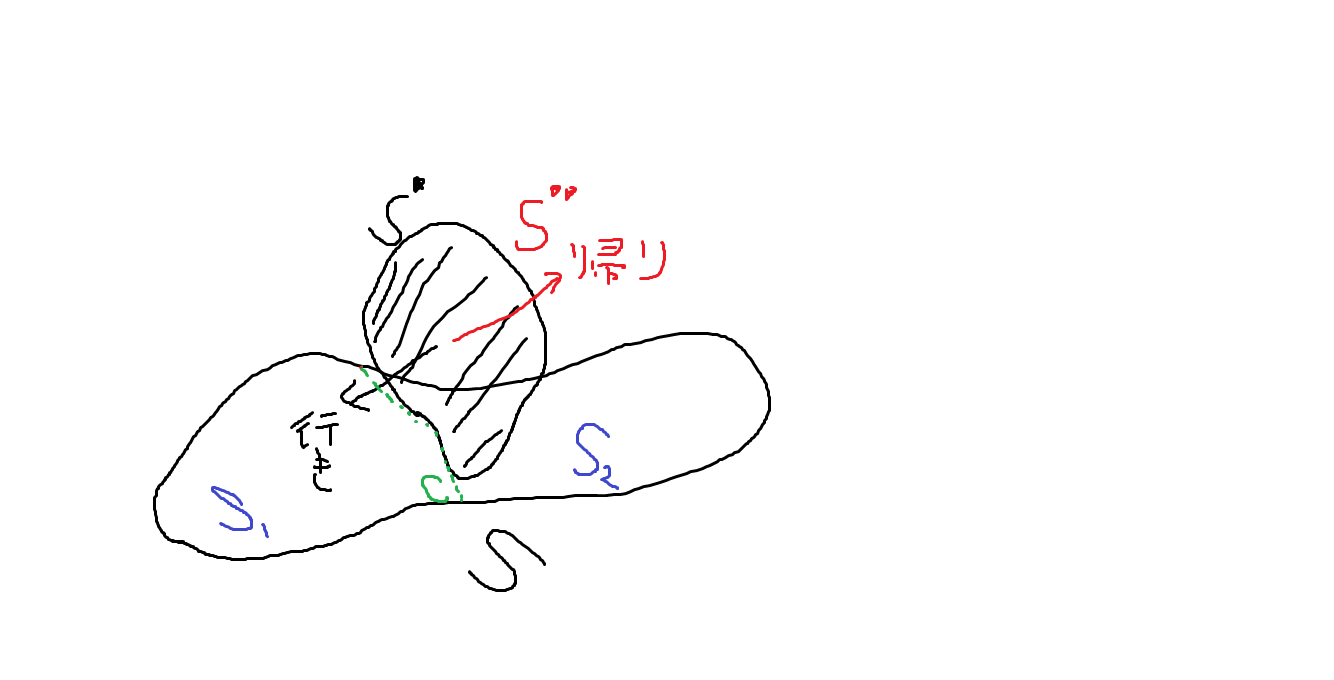
\includegraphics[width=10cm]{Figure/SurfaceAdd.png}
  \end{center}
\end{figure}

さらに, $S^\prime$と, 形状, 位置が全く同じだが, 法線方向が逆, すなわち, 表裏の定義が反対の面$S^{\prime\prime}$を定義する. 
このとき, 全ての面での積分結果は, 
\begin{eqnarray}
  \int_{S_1 S^\prime S^{\prime\prime} S_2}\mbold{A}\cdot\mbold{n}dS 
  && = \int_{S_1}\mbold{A}\cdot\mbold{n}dS + \int_{S_2}\mbold{A}\cdot\mbold{n}dS 
  + \int_{S^\prime}\mbold{A}\cdot\mbold{n}dS + \int_{S^\prime\prime}\mbold{A}\cdot\mbold{n}dS \nonumber \\
  && = \int_{S}\mbold{A}\cdot\mbold{n}dS
  + \int_{S^\prime}\mbold{A}\cdot\mbold{n}dS + \int_{S^\prime\prime}\mbold{A}\cdot (-\mbold{n})dS \nonumber \\
  && = \int_{S}\mbold{A}\cdot\mbold{n}dS
\end{eqnarray}

となり, 結果が変わらない. 

\section{lemma2 : 閉曲面が囲む領域をある面で切断, 分割すると, 元の閉曲面上での積分は, 各領域のを囲む閉曲面での積分の和になる}
閉曲面$S$が囲む領域$V$を, 図のように$V_1$と$V_2$に二分割するように, 曲面$S_3$を定める. 
\begin{figure}[htbp]
  \begin{center}
    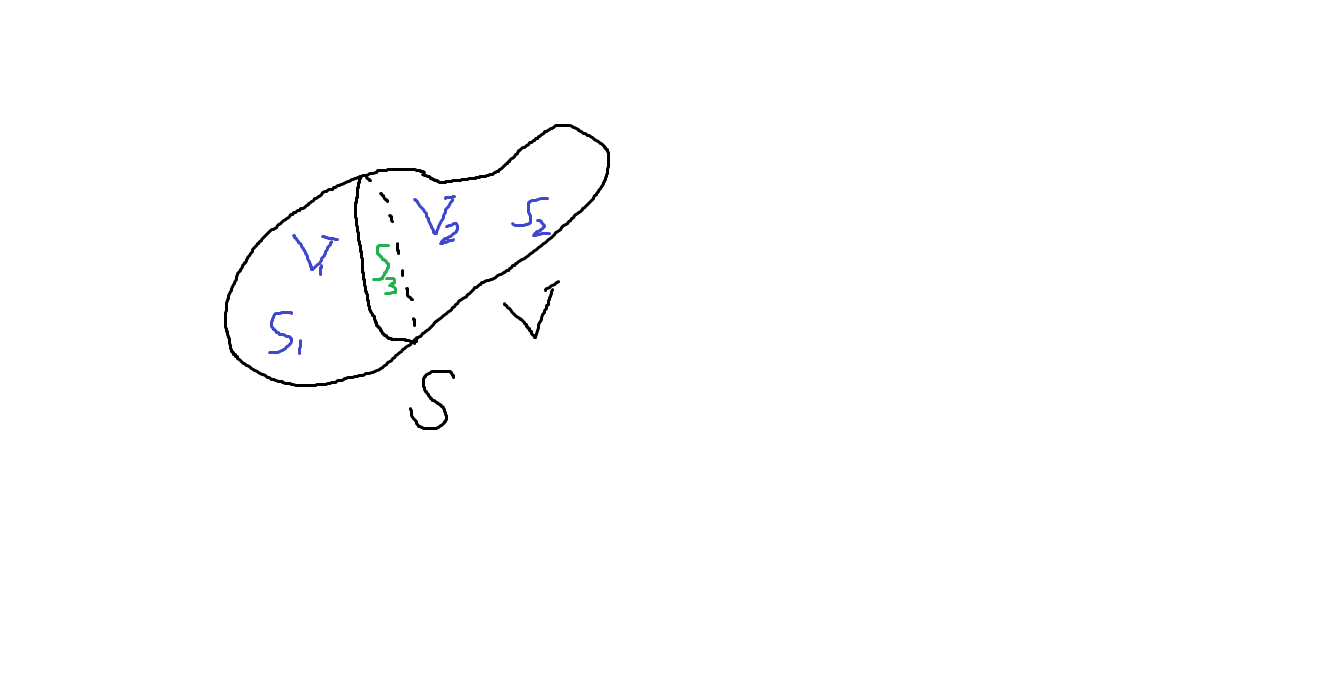
\includegraphics[width=10cm]{Figure/ClosedSurface.png}
  \end{center}
\end{figure}

閉曲面$S$は, $S_3$が持つ境界線により, $S_1$と$S_2$に分けられる. このとき, $S_3$は, $V_1$の外側に法線を取ることにし, $S_3$と同じ面だが, 法線ベクトルが, $V_2$の外側を向く$S_4$を定義すると, これは, $S_3$と$S_4$は, 表裏が逆の面であり, lemma1によれば, 元の$S$での面積分は, $S_3$と, $S_4$を加えた領域での積分結果と変わらない. 
従って, 
\begin{equation}
  \int_S \mbold{A}\cdot \mbold{n} dS
  = \int_{S_1} \mbold{A}\cdot \mbold{n} dS 
  + \int_{S_3} \mbold{A}\cdot \mbold{n} dS 
  + \int_{S_2} \mbold{A}\cdot \mbold{n} dS
  + \int_{S_4} \mbold{A}\cdot \mbold{n} dS
  = \int_{S_1 S_3} \mbold{A}\cdot \mbold{n} dS + \int_{S_2 S_4} \mbold{A}\cdot \mbold{n} dS
\end{equation}

ここで, 第1項に注目すると, $S_1$と$S_3$で作られる面は, $V_1$を囲む閉曲面であり, 同様に, 第2項は$V_2$を囲む閉曲面であり, これらは, 分割された領域ごとに面積分したものの和に他ならない. 

このような操作と, 積分領域の分割を, 任意の回数続けていくことにより, $S$に囲まれた領域を任意の形状に分割することができ, 
全領域の面積分の和, という形になる. 

\section{本証明}
対象となる領域$V$を, 直交する平行な平面で等間隔に格子状に分割すると, $S$のごく近くの領域を除き, 全ての領域が, 直方体になるように切断できる. 
図のような, ある分割領域での面積分を考える. 
\begin{figure}[htbp]
  \begin{center}
    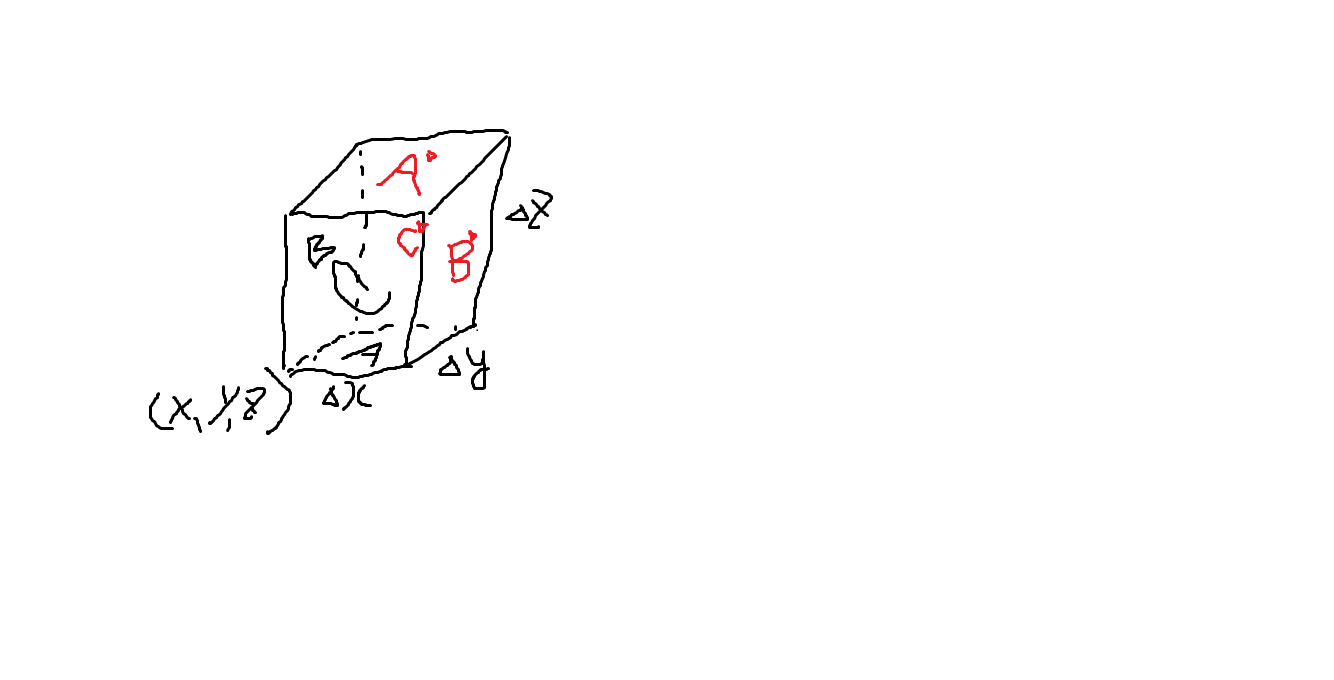
\includegraphics[width=10cm]{Figure/SmallVolume.png}
  \end{center}
\end{figure}

$(x, y, z)$を通り, $xy$面に平行な面を$A$, $yz$面に平行な面を$B$, $xz$面に平行な面を$C$とし, 
同様に$(x + \Delta x, y + \Delta y, z + \Delta z)$を通る面を, $A^\prime$, $B^\prime$, $C^\prime$とする. 
法線ベクトルの向きに気を付けながら, 
\begin{subequations}
  \begin{eqnarray}
    && \int_A \mbold{A}\cdot \mbold{n}dS = \int_x^{x + \Delta x}dp \int_y^{y + \Delta y}dq (-A_z(p, q, z)) \\
    && \int_B \mbold{A}\cdot \mbold{n}dS = \int_y^{y + \Delta y}dp \int_z^{z + \Delta z}dq (-A_x(x, p, q)) \\
    && \int_C \mbold{A}\cdot \mbold{n}dS = \int_x^{x + \Delta x}dp \int_z^{z + \Delta z}dq (-A_y(p, y, q)) \\
    && \int_{A^\prime} \mbold{A}\cdot \mbold{n}dS = \int_x^{x + \Delta x}dp \int_y^{y + \Delta y}dq A_z(p, q, z + \Delta z) \\
    && \int_{B^\prime} \mbold{A}\cdot \mbold{n}dS = \int_y^{y + \Delta y}dp \int_z^{z + \Delta z}dq A_x(x + \Delta x, p, q) \\
    && \int_{C^\prime} \mbold{A}\cdot \mbold{n}dS = \int_x^{x + \Delta x}dp \int_z^{z + \Delta z}dq A_y(p, y + \Delta y, q) 
  \end{eqnarray}
\end{subequations}

これらをすべて足し, 同じ成分同士で整理すると, 
\begin{eqnarray}
  && \int_{ABCA^\prime B^\prime C^\prime} \mbold{A}\cdot \mbold{n}dS \nonumber \\
  && = \int_x^{x + \Delta x}dp \int_y^{y + \Delta y}dq \frac{\partial A_z(p, q, z)}{\partial z}\Delta z \nonumber \\
  && + \int_y^{y + \Delta y}dp \int_z^{z + \Delta z}dq \frac{\partial A_x(x, p, q)}{\partial x}\Delta x \nonumber \\
  && + \int_x^{x + \Delta x}dp \int_z^{z + \Delta z}dq \frac{\partial A_y(p, y, q)}{\partial y}\Delta y 
\end{eqnarray}

ここで, $A_z$を, $(x, y, z)$を中心にTaylor展開すると, 
\begin{equation}
  A_z(p, q, z) = A_z(x, y, z) + \frac{\partial A_z}{\partial x}(p - x) + \frac{\partial A_z}{\partial y}(q - y)
\end{equation}
を利用すると, 積分が実行でき, 同一微少量の二次以上を無視すると, 
\begin{equation}
  \int_x^{x + \Delta x}dp \int_y^{y + \Delta y}dq \frac{\partial A_z(p, q, z)}{\partial z}\Delta z
  = \frac{\partial A_z(x, y, z)}{\partial z}\Delta x \Delta y \Delta z
\end{equation}
同様に他の成分も計算すれば, 
\begin{eqnarray}
  \int_{ABCA^\prime B^\prime C^\prime} \mbold{A}\cdot \mbold{n}dS
  && = \frac{\partial A_x(x, y, z)}{\partial x}\Delta x \Delta y \Delta z
  + \frac{\partial A_y(x, y, z)}{\partial y}\Delta x \Delta y \Delta z
  + \frac{\partial A_z(x, y, z)}{\partial z}\Delta x \Delta y \Delta z \nonumber\\
  && = \divg\mbold{A} \Delta x \Delta y \Delta z
\end{eqnarray}
これを, 大量に分割した, $V$内の各直方体について足し合わせ, 分割サイズの無限小極限を取るので, 
これはすなわち, 体積積分となり, Gaussの定理が成立する. 

この定理は, いわば領域内で発生したものは, 発生した者同士で打ち消しあった結果, 打ち消しきれなかった成分は, 
領域の表面を貫いて出てくる成分と, 総量として一致する, ということを言っており, さらに, 
発生したものの影響のうち, 表面に沿った成分になるものは, 全て打ち消しあうことも意味している. 





\end{document}
